Keeping a lattice with $N=256$ and $a=0.25$ as a case study, we computed the correlation functions $\ct$ (equation \ref{eqn:bestestim})
using $N_{bin}=10000$ bins of dimension $D_{bin}=500$.

Figures \ref{fig:corr} and \ref{fig:errcorr} show the correlators and their error.
\begin{figure}[h!]
\centering
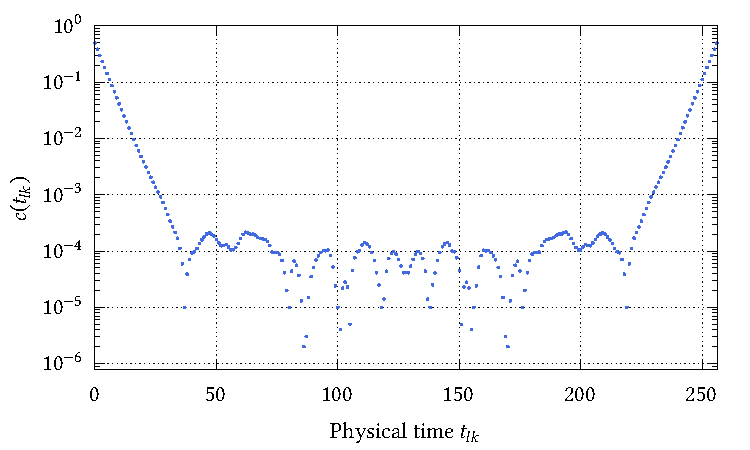
\includegraphics[width=\linewidth]{corr.pdf}
\caption{\label{fig:corr}Logarithmic plot of the correlators as a function of physical time. In this plot we highlight their symmetry with respect to $\t=128$,
more generally they are expected to be symmetric with respect to $\nicefrac{N}{2}$.}
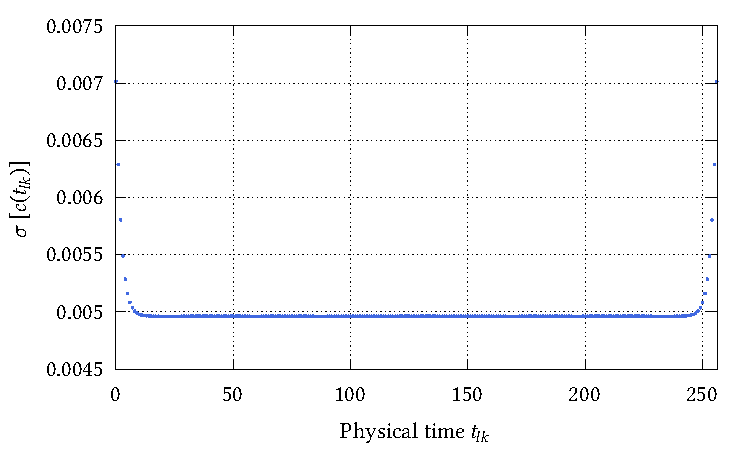
\includegraphics[width=\linewidth]{error}
\caption{\label{fig:errcorr}Standard error on the correlators. When $\lk$ is large, since $\ct$ is exponentially decreasing (equation \ref{eqn:correlators}), the error (equation \ref{eqn:bestvariance}) is dominated by
$\ev{x_{l}^{2}x_{k}^{2}}$ which is constant (equation \ref{eqn:xlxkq}).} 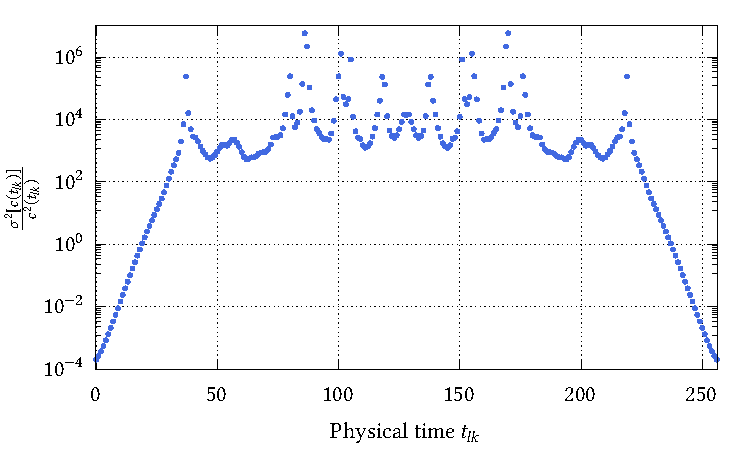
\includegraphics[width=\linewidth]{relerr.pdf}
  \caption{\label{fig:relerr}Logarithmic plot of the relative error squared. The exponential increase when $\lk$ grows but $\nicefrac{N}{2}\gg\lk$ is a manifestation of the so called exponential problem.}

\end{figure}
\\
We note that the plots demonstrate the expected features discussed in subsection \ref{subsec:purpose}: the correlators are symmetric with respect to the central site of the lattice (equation \ref{eqn:correlators}) and the error is constant when the distance between the lattice sites is large enough (equation \ref{eqn:varmatrix}).
Specifically, the errors cluster around $\sigma[\ct] = 0.004962$, which is the value we expect from the square root of equation \ref{eqn:varmatrix} for a lattice of spacing $a=0.25$ on which we considered $N_{bin}=10000$ configurations. Even though this is not enough to draw any definitive conclusions on $|\mel{\tilde{E_{0}}}{\x^{2}}{\tilde{E_{0}}}|$, as that would take a deeper analysis which is outside the scope of this experiment, we take it as a strong check of our results.
The symmetry allows us to discard correlators that depend on $\t > \nicefrac{N}{2}$ when computing $\DEt$ and $\matb$, as $c(\nicefrac{N}{2}+i)$ is identically equal to $c(\nicefrac{N}{2}-i)$ for any give site $i$.

Another expected feature, showcased by figure \ref{fig:relerr}, is the behaviour of the relative error. This is a manifestation of the exponential problem (equation \ref{eqn:relerr}) and will limit the number
of useful correlators in the following analysis.
